\documentclass[a4paper,12pt,portrait]{book}	  
\title{Mathematik f\"ur Physiker I+II}
\author{Friedemann Schuricht\\ \\ \"ubertragen von\\Lukas K\"orber und Friedrich Zahn}
\date{Wintersemester 2014/2015}

  
\usepackage[ngerman]{babel}	    
\usepackage[utf8]{inputenc}
\usepackage[titles]{tocloft}
\usepackage{amsmath}
\usepackage{mathtools}
\usepackage{amsthm}	 
\usepackage{graphicx}      
\usepackage{fancyhdr}
\usepackage{xcolor}
\usepackage[upright]{fourier}
\usepackage[frak=mma]{mathalfa}
\usepackage{sectsty}
\usepackage{lipsum}
\usepackage{bm}


%layout options
\sectionfont{\color{hblue}}
\chapterfont{\color{dblue}}
\pagestyle{headings}
\setlength\parindent{0pt}
\numberwithin{equation}{section}

\renewcommand\theequation{\maybe{\arabic{chapter}}\arabic{section}.\arabic{equation}}
\DeclareRobustCommand\maybe[1]{\ifnum#1=\value{chapter}\relax\else\uppercase\expandafter{\romannumeral#1}.\fi}

\renewcommand*\cftchapnumwidth{0.9cm}
\renewcommand{\thechapter}{\Roman{chapter}} 

\renewcommand*\cftsecnumwidth{0.7cm}
\renewcommand*\thesection{\arabic{section}}

%differential operators
\newcommand{\diff}[2]{\frac{\mathrm{d}{#1}}{\mathrm{d}{#2}}}
\newcommand{\ddiff}[2]{\frac{\mathrm{d}^2{#1}}{\mathrm{d}{#2}^2}}
\newcommand{\dddiff}[2]{\frac{\mathrm{d}^3{#1}}{\mathrm{d}{#2}^3}}
\newcommand{\ndiff}[2]{\frac{\mathrm{d}^n{#1}}{\mathrm{d}{#2}^n}}
\newcommand{\pdiff}[2]{\frac{\partial{#1}}{\partial{#2}}}
\renewcommand{\div}{\mathrm{div\ }}
\newcommand{\rot}{\mathrm{rot\ }}
\newcommand{\grad}{\mathrm{grad\ }}

%hilbert operators
\newcommand{\bra}[1]{\left\langle #1 \right|}
\newcommand{\ket}[1]{\left| #1 \right\rangle}
\newcommand{\lara}[1]{\left\langle #1 \right\rangle}
\newcommand{\scap}[2]{\left\langle #1 \ \middle| \ #2\right\rangle}
\newcommand{\exlara}[3]{\left\langle #1 \ \middle| \ #2 \ \middle| \ #3\right\rangle}

%various operators
\newcommand{\graph}{\text{graph\ }}
\newcommand{\rang}{\text{rang\ }}
\renewcommand{\sup}{\text{sup\ }}
\renewcommand{\inf}{\text{inf\ }}
\renewcommand{\dim}{\text{dim\ }}
\renewcommand{\ker}{\text{ker\ }}
\renewcommand\qedsymbol{$\textbf{q.e.d.}$}
\usepackage{xcolor}
\usepackage{amsthm}	 


\definecolor{dblue}{HTML}{183CE0}
\definecolor{hblue}{HTML}{0E75F7}

\newtheoremstyle{theoremstyle} % name
    {\topsep}                    % Space above
    {\topsep}                    % Space below
    {\upshape}                   % Body font
    {}                           % Indent amount
    {\sffamily\bfseries}                   % Theorem head font
    {}                          % Punctuation after theorem head
    {.5em}                       % Space after theorem head
    {\thmname{#1}\thmnumber{ #2}\thmnote{ (#3)}}  % Theorem head spec (can be left empty, meaning ‘normal’)

\theoremstyle{theoremstyle}
\newtheorem{theo}{Theorem}[section]	% please use "theorem"
\newtheorem{sa}[theo]{Satz}			% please use "satz"
\newtheorem{lem}[theo]{Lemma}		% please use "lemma"
\newtheorem{folgerung}[theo]{Folgerung}
\newtheorem*{definition}{Definition}
\newtheorem{beispiel}{Beispiel}
\newtheorem*{beispiel*}{Beispiel}

\newenvironment{theorem}
	{\par\nobreak\vfil\penalty0\vfilneg
   \vtop\bgroup\color{dblue}\noindent\rule{420pt}{2pt}\vspace{5pt}\begin{theo}}
	{\end{theo}\rule{50pt}{1pt}\color{black}\par\xdef\tpd{\the\prevdepth}\egroup
   \prevdepth=\tpd}
\newenvironment{satz}
	{\par\nobreak\vfil\penalty0\vfilneg
   \vtop\bgroup\color{dblue}\noindent\rule{420pt}{2pt}\vspace{5pt}\begin{sa}}
	{\end{sa}\rule{50pt}{1pt}\color{black}\par\xdef\tpd{\the\prevdepth}\egroup
   \prevdepth=\tpd}
\newenvironment{lemma}
	{\par\nobreak\vfil\penalty0\vfilneg
   \vtop\bgroup\color{dblue}\noindent\rule{420pt}{2pt}\vspace{5pt}\begin{lem}}
	{\end{lem}\rule{50pt}{1pt}\color{black}\par\xdef\tpd{\the\prevdepth}\egroup
   \prevdepth=\tpd}
	
\begin{document}
\maketitle
\tableofcontents
\setcounter{chapter}{7}
\chapter*{Überblick}
Diese Vorlesung wird sich mit folgenden Tehmen befassen:
    \begin{enumerate}
    \item \textbf{Integration auf Mannigfaltigkeiten}
    \item \textbf{Differenzialgleichungen}, sowohl gewöhnlich, als auch partiel
    \item \textbf{Funktionalanalysis} in Banach- und Hilberträumen (insbesondere
    unendlich dimensionale Räume z.B. von Folgen und Funktionen)
    \item \textbf{Funktionstheorie}, der Theorie von komplexwertigen Funktionen
    und z.B. $\mathbb{C}$-Differenzierbarkeit
    \end{enumerate}

\chapter{Integration auf Mannigfaltigkeiten}
\emph{Literaturtipp:} Königsberger Analysis 2, Springer
\setcounter{section}{28}

\section{Mannigfaltigkeiten}
Sei $\varphi\in C^q(V,\mathbb{R}^n)$ mit $q\in\mathbb{N}_{\geq 1}$, 
also $q$-fach stetig differenzierbar, wobei $V\subset\mathbb{R}^d$ offen ist, 
dann heißt $\varphi$ \textbf{regulär}, falls
    \begin{equation}
    \varphi'(x):\mathbb{R}^d\rightarrow\mathbb{R}^n \ \text{regulär (d.h. injektiv)}
    \end{equation}
Falls $\varphi$ regulär für alle $x\in V$ ist, heißt es auch 
\textbf{regulär auf V} beziehungsweise \\
\textbf{reguläre $C^q$-Parametrisierung} (manchmal auch $C^q$-Immersion). \\
$V$ ist dann der \textbf{Parameterbereich} von $\varphi$.\\
\emph{Bemerkung:} $\varphi(V)$ wird selten auch \textbf{Spur} von $\varphi$ genannt.\\
\linebreak
\linebreak
Aus der Linearen Algebra wissen wir, dass aus (29.1) sofort 
    \begin{equation}
    d\leq n
    \end{equation}
folgt. Dies sei in Kapitel VIII immer erfüllt! (29.2) ist außerdem äquivalent dazu, dass 
$\rang \varphi'(x)=d$.\\
    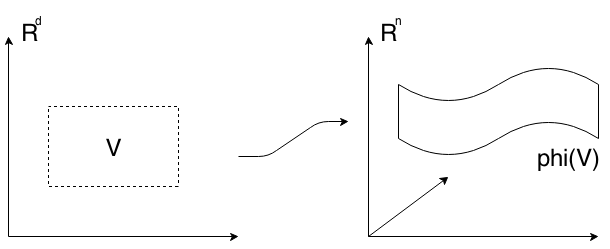
\includegraphics[scale=0.5]{pictures/MA2_0001}

\begin{beispiel}[reguläre Kurven $\varphi:I\subset\mathbb{R}\rightarrow\mathbb{R}^n$]
Dabei ist $I$ offen und der Tagentialvektor nirgendwo identisch mit dem Nullvektor, also 
$\varphi'(x)\neq 0$

\begin{enumerate}
    \item $\varphi:(0,2\pi)\rightarrow\mathbb{R}^2$ mit $\varphi(t)=\begin{pmatrix}
        \cos kt \\ \sin kt
    \end{pmatrix}$ und $k\in\mathbb{N}_{\geq 2}$\\

\begin{center}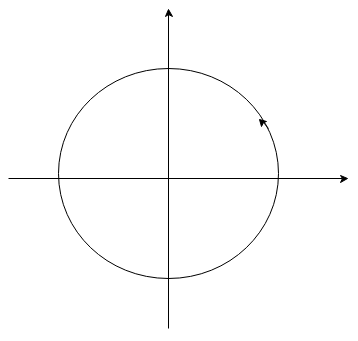
\includegraphics[scale=0.3]{pictures/MA2_0002}\\ 
\end{center}

Der Einheitskreis wird hier k-mal durchlaufen. 
Da $\varphi'(x)\neq 0$, ist $\varphi$ regulär.
\item $\varphi(-\pi,\pi)\rightarrow\mathbb{R}^2$ mit $\varphi(t)=(1+2\cos t)
    \begin{pmatrix}
    \cos t \\ \sin t
    \end{pmatrix}$\\

\begin{center}
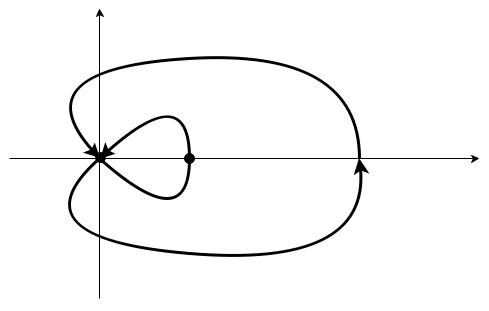
\includegraphics[scale=0.3]{pictures/MA2_0003}\\
\end{center}

$\varphi(\pm\frac{2\pi}{3})=
    \begin{pmatrix}
    0 \\ 0
    \end{pmatrix}
$, $ 
\varphi(0)=
    \begin{pmatrix}
    3 \\ 0
    \end{pmatrix}
$\\$
    \begin{pmatrix}
    1 \\ 0
    \end{pmatrix} $ 
\ gehört \textbf{nicht} zur Kurve ("$=\varphi(\pm\pi)$") und $\varphi$ ist regulär.

\item $\varphi:(-1,1)\rightarrow\mathbb{R}^2$ \ mit \ $\varphi(t)=\begin{pmatrix}
    t^3 \\ t^2
\end{pmatrix}$ \ ist wegen $\varphi'(0)=0$ \ \textbf{nicht} regulär\\

    \begin{center}
    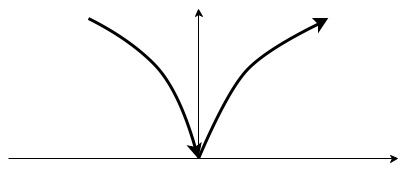
\includegraphics[scale=0.3]{pictures/MA2_0004}
    \end{center}

\end{enumerate}

\end{beispiel}
\ \linebreak

\begin{beispiel}[Parametrisierung von Graphen]
Sei $f\in C^q(V,\mathbb{R}^{n-d})$,\\
$V\subset\mathbb{R}^d$. Betrachtet wird $\varphi:V\rightarrow\mathbb{R}^n$ mit $\varphi(x)=(x,f(x))$\\
    \begin{center}
    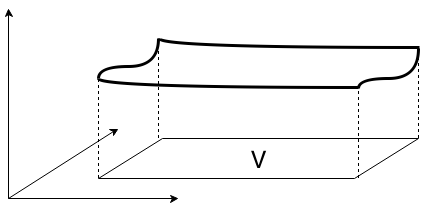
\includegraphics[scale=0.5]{pictures/MA2_0005}\\
    \end{center}
$\varphi$ ist regulär, da offenbar $\varphi\in C^q(V,\mathbb{R}^n)$ 
und $\varphi'=
    \begin{pmatrix} 
    id^d \\ 
    f'(x)
    \end{pmatrix}     
\in \mathbb{R}^{n \times d}$ \ ist.\\
\linebreak
\end{beispiel}

Es folgt eine Wiederholung zur \textbf{Relativtopologie} (vgl. Kapitel 14). Wir wissen, dass $U\subset M$ genau dann offen bezüglich $M$ ist, wenn es ein $\tilde{U}\subset\mathbb{R}^n$ gibt, dass offen ist, und das $U=\tilde{U}\cap M$ erfüllt. Später wird $M$ eine Mannigfaltigkeit sein und wir werden untersuchen, was in ihr offen ist.\\

\begin{center}
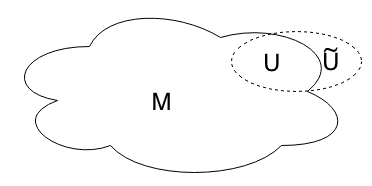
\includegraphics[scale=0.5]{pictures/MA2_0006}\\
\end{center}
Auf dieser Grundlage lässt sich auch der Begriff der \textbf{Umgebung} definieren:\\
$U\subset M$ heißt nämlich genau dann Umgebung von $u\in M$ bezüglich $M$, wenn es ein bezüglich $M$ offenes $U_0\subset M$ gibt, in dem $u$ liegt und das Teilmenge von $U$ ist.\linebreak\linebreak
\newpage
\textbf{\textsf{Beispiel für}} \ $M\subset\mathbb{R}^n$.\\

\begin{center}
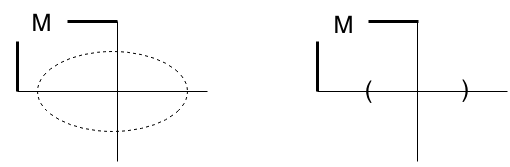
\includegraphics[scale=0.5]{pictures/MA2_0007}\\
\end{center}
\hspace{70pt} offen bzgl. M \hspace{70pt} nicht offen bzgl. M\\

\begin{definition}[Mannigfaltigkeiten]
Wir nennen $M\subset\mathbb{R}^n$ eine \textbf{d-dimensionale $C^q$-Mannigfaltigkeit} ($q\in\mathbb{N}_{\geq 1}$), falls

\begin{enumerate}
\item es für alle $u\in M$ eine (offene) Umgebung $U$ von $u$ bezüglich $M$ gibt und
\item es eine reguläre $C^q$-Parametrisierung $\varphi:V\subset\mathbb{R}^d\rightarrow\mathbb{R}^n$ ($V$ ist offen) existiert, die homöomorph ist und in die Mannigfaltigkeit abbildet (also \  $\varphi(V)=U$).
\end{enumerate}

\emph{Wiederholung: Eine stetige Abbildung heißt homöomorph, falls eine Umkehrabbildung existiert, die auch stetig ist.}\\
\end{definition}

In der Literatur wird $M$ auch manchmal als $C^q$-\emph{Unter}mannigfaltigkeit bezeichnet. Wir werden jedoch später zeigen, dass die verschiedenen Definitionen von Mannigfaltigkeiten gleichwertig sind.\\
Da ab jetzt immer hauptsächlich $C^1$-Mannigfaltigkeiten auftauchen werden, werden wir diese in Zukunft einfach "Mannigfaltigkeiten" nennen.\\

\begin{center}
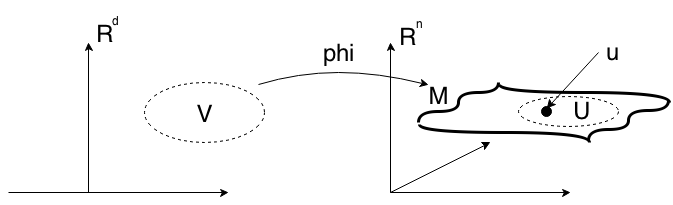
\includegraphics[scale=0.5]{pictures/MA2_0008}\\
\end{center}

Die Umkehrabbildung $\varphi^{-1}$ beziehungsweise ($\varphi^{-1}, U$) nennt man die \textbf{Karte} von $M$ um $u\in M$, wobei $U$ das zugehörige \textbf{Kartengebiet}, $\varphi$ selbst die Parametrisierung und $V$ der Parameterbereich ist.\\
Karten können eine Mannigfaltigkeit jedoch nur lokal beschreiben. Aus diesem Grund führt man den Begriff des Atlas, der eine globale Beschreibung ermöglicht, ein:\\
Die Menge $\{\varphi^{-1}_\alpha | \alpha\in A\}$ heißt \textbf{Atlas} der Mannigfaltigkeit M, falls die zugehörigen Kartengebiete $U_\alpha$ jene vollständig überdecken.\\
\linebreak
Weiterhin wichtig ist der Begriff der sogenannten \textbf{Einbettung}, bei der es sich um eine reguläre Parametrisierung handelt, die homöomorph ist. Wir vereinbaren, dass es sich im folgenden bei allen Parametrisierungen von Mannigfaltigkeiten stets um Einbettungen handelt.
\begin{beispiel}[Beweise bitte Selbstudium]\ \\

\begin{enumerate}
\item Der Kreis aus Beispiel 1.1 ist eine 1-dimensionale $C^\infty$-Mannigfaltigkeit, obwohl der Kreis k-fach durchlaufen wird. Der Atlas benötigt mindestens zwei Karten.
\item Die Kurven aus Biespiel 1.2 und 1.3 sind keine Mannigfaltigkeiten, da $\varphi$ nicht überall homöomorph ist.
\item Jedes offene $M\subset\mathbb{R}^n$ ist eine n-dimensionale $C^\infty$-Mannigfaltigkeit mit $\{id\}$ als Atlas.
\end{enumerate}
\end{beispiel}

\begin{beispiel} Sei $M:=\graph f$ aus Beispiel 2. Offenbar ist 
$\varphi:V\subset\mathbb{R}^d\rightarrow M\subset\mathbb{R}^n$ 
eine Einbettung. Das macht $M$ zu einer d-dimensionalen $C^q$-Mannigfaltigkeit.
\end{beispiel}

\begin{beispiel}
Sei $f:D\subset\mathbb{R}^n\rightarrow\mathbb{R}^{n-d}$ ($D$ offen) q-fach stetig differenzierbar für $q\geq 1$. Offenbar ist

\begin{equation}
\rang f'(u)=n-d \ \ \ \ \ \ \ \forall u\in D
\end{equation}
Wir nennen $M=\{u\in D \ | \ f(n)=0\}$ die Niveaumenge von $f$\\

\begin{center}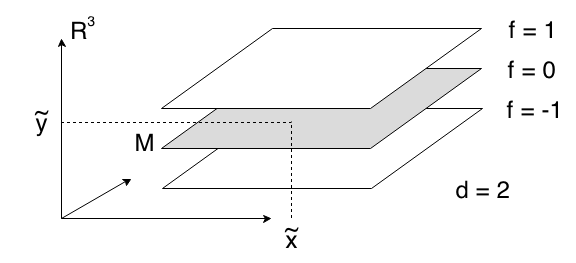
\includegraphics[scale=0.5]{pictures/MA2_0009}\\
\end{center}

Fixieren wir $\tilde{u}=(\tilde{x},\tilde{y})=(x_1,...,x_d,y_1,...,y_{n-d})\in M$
, so sehen wir mit (29.3) und eventuellen Koordinatenvertauschungen, dass 
$f(\tilde{x},\tilde{y})$ regulär ist. Der \emph{Satz über implizite Funktionen}
sichert uns nun, dass es eine Umgebung $V\subset\mathbb{R}^d$ von $\tilde{x}$, 
eine Umgebung $W\subset\mathbb{R}^{n-d}$ von $\tilde{y}$ und ein 
$\psi:V\rightarrow W\in C^q(V,W)$ gibt, das $(x,\psi(x))\in M$ erfüllt und homöomorph ist.\\
Es folgt, dass $\varphi:V\subset\mathbb{R}^d\rightarrow\mathbb{R}^n$ mit
$\varphi(x)=(x,\psi(x))$ eine homöomorphe, reguläre Einbettung  und $\varphi(V)$ 
Umgebung von $\tilde{u}\in M$ bezüglich von $M$ ist. Daraus können wir nun schließen, 
dass $M$ eine d-dimensionale $C^q$-Mannigfaltigkeit ist.\\
\linebreak
\emph{Bemerkung: $M=\graph f$ und $M=\{f=0\}$ sind grundlegende Konstruktionen 
für Mannigfaltigkeiten. \textbf{Lokal} ist jede Mannigfaltigkeit von dieser Gestalt!}
\end{beispiel}

\begin{sa}[lokale Darstellung einer Mannigfaltigkeit als Graph]
\mbox{} \\
Sei $M \subset \mathbb{R}^{n}$ eine d-dimensionale $C^{q}$-Mannigfaltigkeit. \\
$\Longleftrightarrow \forall u \in M \subset \mathbb{R}^n $ existiert eine Umgebung
$U$ von $u$  bezüglich $M$, $W \subset \mathbb{R}^n $ offen, 
$f \in C^q (W, \mathbb{R}^{n-d})$ und eine Permutation $\pi$ von Koordinaten in
$\mathbb{R}^n $ mit $ \psi (W) = U $ für $ \psi (v) \coloneqq \psi (v, f(v)) 
\forall v \in W $ (das heißt $U$ ist Graph von f).
\end{sa}

\textbf{somit:} $M$ ist $C^q$-Mannigfaltigkeit genau dann, wenn $M$ lokaler Graph
einer $C^q$-Funktion $f$ ist (vergleiche Beispiel 2 und 4).

\begin{proof}

$"\Leftarrow"$: folgt aus Beispielen 2 und 4. \\
$"\Rightarrow"$: fixiere $\tilde{u} \in M $, sei $\varphi : \tilde{V} \in \mathbb{R}^d
\rightarrow \tilde{U} \subset \mathbb{R}^n $ und der zugehörige $C^q$-Parameter 
$\tilde{u} = \varphi (\tilde{x})$ \\
$\varphi' (x)$ ist regulär $\xRightarrow{\text{ evtl. $\pi$ der Zeilen }} \varphi_I ' 
(\tilde{x}) \subseteq \mathbb{R}^{d \times d} $ ist regulär für $\varphi (x) =
    \begin{pmatrix}
    \varphi_I (x) \left[ \in \mathbb{R}^d \right]\\
    \varphi_{II} (x) \left[ \in \mathbb{R}^{n-d} \right]
    \end{pmatrix}
$ \\
Zerlege $u = \pi (v,w) $ mit $v \in \mathbb{R}^d $, 
d.h. $\tilde{u} = \pi (\tilde{v},\tilde{w})$

\textbf{Skizzen fehlen!}\\
$\xRightarrow{\text{Theorem über inverse Fkt.}} \exists V \subset \tilde{V} $ offen,
$\tilde{x} \in V, W \subset \mathbb{R}^d $ offen, $\tilde{v} \in W $
mit $\varphi_I ^{-1} : W \rightarrow V $ Homöomorphismus und $C^q$-Abbildung,
$\varphi_I ^{-1} (\tilde{v}) = \tilde{x} $ \\
mit $f(v) \coloneqq \varphi_{II} \left(\varphi_I ^{-1} (v)\right) \forall v \in W $ ist 
$f \in C^q \left(W, \mathbb{R}^{n-d}\right) $ \\
und $\psi (v) \coloneqq \varphi \left(\varphi_I ^{-1} (v) \right) =
\left( \varphi_I \left(\varphi_I ^{-1} (v) \right( ,
\varphi_{II} \left(\varphi_I ^ {-1} (v) \right) \right) = \pi \left(v, f(v)\right) $ \\
$\Rightarrow \psi (\tilde{v}) = \pi (\tilde{v}, \tilde{w}) = \tilde{u},
\psi (w) = \varphi (v) \in M \\
\varphi : \tilde{V} \rightarrow \tilde{U} $ ist Homöomorphismus \\
$\Rightarrow \varphi (v) $ ist offen in $M$ \\
$ \Rightarrow U \coloneqq \psi (W) $ ist offen bezüglich $M$
$\Rightarrow U $ ist Umgebung von $\tilde{u} $ bezüglich $M$ \\
$\xRightarrow{\tilde{u} \text{ beliebig}} $ Behauptung. 

\end{proof}

\begin{sa}[Charakterisierung von Mf mit umgebendem Raum]
\mbox{} \\
$M \subset \mathbb{R}^n $ sei d-dimensionale $C^q$-Mannigfaltigkeit. \\
$\Longleftrightarrow \forall u \in M $ existiert eine Umgebung $\tilde{U}$ von $u$ 
bezüglich $\mathbb{R}^n$, \\
$\tilde{V} \subset \mathbb{R}^n $, 
$\tilde{\psi}: \tilde{U} \rightarrow \tilde{V} $ wobei $\tilde{\psi} $ 
ein $C^q$-Diffeomorphismus ist und 
    \begin{equation*}
    \tilde{\psi} \left( \tilde{U} \cap M \right) =
    \tilde{V} \cap \left( \mathbb{R}^d \times {0} \right) 
    \end{equation*}

\textbf{Skizzen fehlen!}
\end{sa}

\textbf{Bemerkung:} Diese Charakterisierung von Mannigfaltigkeiten benutzt den umgebenden Raum und wird häufig als Definition der Mannigfaltigkeit benutzt.    
    
\begin{proof}
$"\Leftarrow"$: $\psi $ eingeschränkt auf $\tilde{U} \cap M $ liefert Karten 
$\Rightarrow$ Behauptung. \\
$"\Rightarrow"$: fixiere $\tilde{u} \in M $, wähle $\tilde{U} \subset M $,
$W \subset \mathbb{R}^d $, $f \in C^q \left( W, \mathbb{R}^{n-d} \right)$ \\
gemäß Satz 29.1 oBdA $\pi = $ \textit{id} \\
zerlege $u = (v,w) \in \mathbb{R}^d \times \mathbb{R}^{n-d}$, 
$\tilde{u} = \left( \tilde{v}, f \left( \tilde{v} \right) \right) $ \\
sei $\hat{U} \coloneqq W \times \mathbb{R}^{n-d} \eqqcolon \hat{V} $,
liefert "Zylinder" aus $U$ und $W$ in Beweis zu Satz 29.1 \\
sei $\tilde{\varphi}: \hat{V} \rightarrow \hat{U} $ mit
$\tilde{\varphi} (v,w) \coloneqq (v, f(v) + w) \Rightarrow \tilde{\varphi} \in C^q $ \\
$\tilde{\varphi}' \left( \tilde{v}, 0 \right) =
    \begin{pmatrix}
    \textit{id}_d & 0 \\
    f'(v)         & \textit{id}_{n-d}
    \end{pmatrix}
$ ist regulär \\
$\xRightarrow{\text{Satz ü. inverse Fkt.}} \exists $ 
Umgebung $ \tilde{U} \subset \hat{U}$ von $\tilde{U}$,
Umgebung $ \tilde{V} \subset \hat{V} $ von $ \left( \tilde{v}, 0 \right) $, sodass \\
$\tilde{\psi} \coloneqq \tilde{\varphi}^{-1} \in C^q \left( \tilde{U}, \tilde{V} \right) $
exisitiert. \\
wegen $\tilde{\varphi} \left( \tilde{V} \cap \left( \mathbb{R}^d \times {0} \right) \right)
= \tilde{U} \cap M $ folgt die Behauptung.
\end{proof}

\begin{folgerung}
Sei $M \subset \mathbb{R}^n$ d-dimensionale $C^q$-Mannigfaltigkeit \\
und $\varphi: V \subset \mathbb{R}^d \rightarrow U \subset M $ Parameter um $u \in M $ \\
$\Longrightarrow \exists \tilde{U}, \tilde{V} \subset \mathbb{R}^n $ offen und 
$\tilde{\varphi} : \tilde{V} \rightarrow \tilde{U} $ 
mit $ U \subset \tilde{U}, V \times {0} \subset \tilde{V} $, \\
$\tilde{\varphi} $ ist $C^q$-Diffeomorphismus und
$\tilde{\varphi} (x, 0) = \varphi (x) \forall x \in V $
\end{folgerung}

\begin{proof}
Folgt aus Beweisen von Satz 29.1 und 29.2
\end{proof}

\begin{theo}[lokale Darstellung von Mf als Niveaumenge]
\mbox{} \\
$M \subset \mathbb{R}^n $ sei d-dimensionale $C^q$-Mannigfaltigkeit. \\
$\Longleftrightarrow \forall u \in M $ existiert eine Umgebing $\tilde{U}$ von $u$
bezüglich $\mathbb{R}^n$ und \\
$f \in C^q \left( \tilde{U}, \mathbb{R}^{n-d} \right)$ 
mit $\textit{rang } f' (u) = n-d $ und \\
$\tilde{U} \cap M = \left\lbrace \tilde{u} \in \tilde{U} | f (\tilde{u}) = 0 \right\rbrace $
\end{theo}

\textbf{somit:} $M$ ist eine $C^q$-Mannigfaltigkeit genau dann, 
wenn $M$ die lokale Niveaumenge einer $C^q$-Funktion $f$ ist. \\

\textbf{Bemerkung:} $c \in \mathbb{R}^{n-d} $ heißt \textit{regulärer Wert} von
$f \in C^q \left( \tilde{U}, \mathbb{R}^{n-d} \right) $, \\
$\tilde{U} \subset \mathbb{R}^n $
offen, falls $\textit{rang } f' (u) = n-d \forall u \in \tilde{U} $ mit $f(u) = c $ \\
Folglich ist $M \coloneqq \left\lbrace u \in \tilde{U} | f(u) = c \right\rbrace $ 
eine d-dimensionale $C^q$-Mannigfaltigkeit, falls $c$ ein regulärer Wert von $f$ ist.

\begin{proof}
$"\Leftarrow":$ gemäß Bsp. 5 erhält man lokale Parametriesierung \\
$\Rightarrow$ Behauptung. \\
$"\Rightarrow":$ fixiere $\tilde{u} \in M$, 
wähle $\tilde{U}, \tilde{V} \subset \mathbb{R}^n, 
\tilde{\psi}: \tilde{U} \rightarrow \tilde{V} $ gemäß Satz 29.2 \\
sei $f \coloneqq \left( \tilde{\psi}_{d+1}, \ldots , \tilde{\psi}_n \right)$,
offenbar $f \in C^q \left(  \tilde{U}, \mathbb{R}^{n-d} \right) $ \\
mit $\tilde{\psi}$ aus dem Beweis zu Satz 29.2:
$\tilde{\psi}' (\tilde{u}) = \tilde{\varphi}' (\tilde{v}, 0)^{-1} $ ist regulär \\
$\Rightarrow f'(\tilde{u}) $ hat vollen Rang, d.h. $\textit{rang } f'(\tilde{u}) = n-d $ \\
nach Konstruktion $ \left\lbrace u \in \tilde{U} | f(u) = 0 \right\rbrace = U \cap M
\Rightarrow $ Behauptung.
\end{proof}

\begin{lem}[Kartenwechsel] 
\mbox{} \\
Sei $M \in \mathbb{R}^n $ d-dimensionale Mannigfaltigkeit \\
und $\varphi_1^{-1}, \varphi_2^{-1} $ Karten mit zugehörigem Kartengebiet 
$U_1 \cap U_2 \neq \emptyset $ \\
$\Longrightarrow 
\varphi_2^{-1} \circ \varphi_1 : \varphi_1^{-1} \left( U_1 \cap U_2 \right)
\rightarrow \varphi_2^{-1} \left( U_1 \cap U_2 \right) $ ist $C^q$-Diffeomorphismus.

\textbf{Skizze fehlt!}
\end{lem}

\begin{proof}
Ersetze $\varphi_1, \varphi_2 $ mit $\tilde{\varphi}_1, \tilde{\varphi}_2 $
gemäß Folgerung 29.3 \\
$\Rightarrow$ Einschränkung von $\tilde{\varphi}_2^{-1} \circ \tilde{\varphi}_1 $
liefert Behauptung. 
\end{proof}

\begin{definition}
Sei $M \subset \mathbb{R}^n $ d-dimensionale Mannigfaltigkeit. \\
Ein Vektor $v \in \mathbb{R}^n $ heißt \textbf{Tangentialvektor} in $u \in M $ an $M$, \\
falls eine stetig differenzierbare Kurve 
$\gamma: (-\delta, \delta) \rightarrow M (\delta > 0) $ exisitiert mit \\
$\gamma (0) = u $ und $\gamma' (0) = v $. \\
Die Menge aller Tangentialvektoren $T_uM$ heißt Tangentialraum.
\end{definition}

\begin{sa}
Sei $M \in \mathbb{R}^n $ eine d-dimensionale Mannigfaltigkeit, \\
$u \in M $, $ \varphi : V \rightarrow U $ der zugehörige Parameter um $u$ \\
$\Longrightarrow T_uM $ ist d-dimensionaler $( \mathbb{R}-) $ Vektorraum und \\
    \begin{equation}
    T_uM = \underbrace{\varphi'(x)}_{L \left( \mathbb{R}^d, \mathbb{R}^n \right) }
    \left( \mathbb{R}^d \right) \text{ für } x = \varphi^{-1} (u) 
    \end{equation}
wobei $T_uM$ unabhängig vom speziellen Parameter $\varphi$ ist.
\end{sa}

\begin{proof}
Sei $\gamma: (-\delta, \delta) \rightarrow M eine C^1$-Kurve mit $\gamma(0) = u $ \\
$\Rightarrow g \coloneqq \varphi^{-1} \circ \gamma $ ist $C^1$-Kurve, 
$g: (-\delta, \delta) \rightarrow \mathbb{R}^d $ mit $ g(0) = x $ und
    \begin{equation*}
    \gamma' (0) = \varphi' (x) g'(0) \text{, } \varphi' (x) \text{ist regulär.}
    \tag{$\spadesuit$}
    \end{equation*}
Offenb. liefert auch jede $C^1$-Kurve $g$ in $\mathbb{R}^d $ durch $x$
eine $C^1$-Kurve $\gamma$ in $M$ mit $(\spadesuit)$ \\
Die Menge aller Tangentialvektoren $g'(0)$ von $C^1$-Kurven $g$ in $\mathbb{R}^d $
ist offenbar $\mathbb{R}^d $ \\
$\Rightarrow $ 
29.4 $ \xRightarrow{\varphi' (x) \text{ ist regulär}} \textit{dim } T_uM = d $ \\
da $(\spadesuit)$ für jeden Parameter $\varphi$ gilt, ist $T_uM$ unabhängig von $\varphi$.
\end{proof}

\textbf{Bemerkung:}
\par \noindent
Man bezeichnet auch $(u, T_uM) \subset M \times \mathbb{R}^n$
als Tangentialraum und \\
$TM = \bigcup\limits_{U \in M} (u, T_uM) \subset M \times \mathbb{R}^n $
als Tangentialbündel.

\begin{beispiel}
Sei $M \subset \mathbb{R}^n $ offen  \\
$\Rightarrow $ $M$ ist ist n-dimensionale Mannigfaltigkeit und 
$T_uM = \mathbb{R}^n \forall u \in M $
\end{beispiel}

\begin{definition}
Sei $M \subset \mathbb{R}^n $ d-dimensinale Mannigfaltigkeit. \\
Ein Vektor $w \in \mathbb{R}^n $ heißt \textbf{Normalenvektor} in $u \in M $ an $M$, falls\\
$\langle w,v \rangle = 0 \forall v \in T_uM $
(d.h. $w \bot v \forall v \in T_uM$) \\
Die Menge aller Normalenvektoren $N_uM = T_uM^{\bot} $ heißt \\
\textbf{Normalenraum} von $M$ in $u$. 
\end{definition}
\begin{satz}
Sei $f\in C^1\left(V,\mathbb{R}^{n-d}\right)$ mit $V$ offen und $c\in\mathbb{R}^{n-d}$ ein regulärer Wert von $f$. Dann ist die Niveaumenge $M\coloneqq\{v\in V \ | \ f(u)=c\}$ eine d-dimensionale Mannigfaltigkeit, für die gilt:
\begin{eqnarray*}
T_uM &=&\{v\in\mathbb{R}^n \ | \ f'(u)v=0\} \ \ \left(=\ker f'(u)\right) \ \ \forall u\in M \\
N_uM&=&\{w\in\mathbb{R}^n \ | \ w=f'(u)^Tv, v\in\mathbb{R}^{n-d}\} \ \ \forall u\in M 
\end{eqnarray*}
Das heißt also, die Spalten von $f'(u)^T$ bilden eines Basis des Normalenraums von $M$.
\end{satz}

\begin{beispiel}
Sei $f=\begin{pmatrix}
f_1 \\ f_2
\end{pmatrix}\in C^1\left(\mathbb{R}^3,\mathbb{R}^2\right)$ und $0\in\mathbb{R}^2$ ein regulärer Wert von $f$. Dann ist
\begin{equation*}
M:=\{u\in\mathbb{R}^3 \ | \underbrace{\ f_1(u)=0, \ f_2(u)=0}_{\text{Schnitt \ zweier \ Flächen}}\}
\end{equation*}
eine 1-dimensionale Mannigfaltigkeit. Dann steht der Gradient $f'_i(u)^T$ senkrecht auf $\{f_i=0\}$. $f'_1(u)^T$ und $f'_2(u)^T$ sind also Normalen zu $M$ in $u$.\\
\begin{center}
	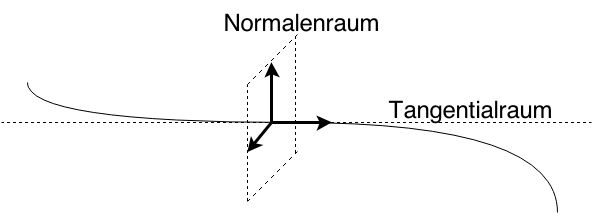
\includegraphics[scale=0.5]{pictures/003-01.png}
\end{center}
$v$ ist hier die Tangente, da $\scap{f'_i(u)^T}{v}=0$ ist (für $i=1,2$).
\end{beispiel}

\begin{proof}
Wir wissen bereits, dass $M$ eine Mannigfaltigkeit ist. Wählen wir nun die $C^1$-Kurve $\gamma$ auf $M$ mit $\gamma(0)=u$ und $\gamma'(0)=v$, so sehen wir, dass $f(\gamma(t))=c \ \forall t$ ist. $f'(u)$ steht senkrecht auf $v$ (also $\scap{f'(u)}{v}=0$) und da $\rang f'(u)=d$ ist, muss $\dim \ker f'(u)=d$ sein. Damit ist die Behauptung für $T_uM$ (wegen $\dim T_uM)=d$) gezeigt.\\
Nun wählen wir $w=f'(u)^T\tilde{v}$ und $w\in T_uM$. Offenbar ist $\scap{w}{v}=\scap{\tilde{v}}{f'(u)v}=0$. Damit ist $w$ im Normalenraum $N_uM$. Da $\rang f'(u)^T=n-d$  und $\dim N_uM=n-d$, folgt die Behauptung.
\end{proof}

\begin{beispiel}
Wir betrachten $M\coloneqq\mathcal{O}(n)=\{A\in\mathbb{R}^{n\times n}\ |\ A^TA=id \}$. 
Es handelt sich dabei um eine $\frac{n(n-1)}{2}$-dimensionale Mannigfaltigkeit von Matritzen. 
Man nennt $\mathcal{O}$ auch \emph{Orthogonale Gruppe} oder \emph{Lie-Gruppe}. 
Sie bildet die Menge aller orthogonale Matrizen des $\mathbb{R}^{n\times n}$. 
Offenbar ist $id$ das neutrale Element der Gruppe. Der Tangentialraum an diesem Element wird auch \emph{Lie-Algebra} genannt:
\begin{equation*}
T_{id}M=\{B\in\mathbb{R}^{n\times n}\ |\ B+B^T=0\}
\end{equation*}
Dies ist die Menge der schiefsymetrischen Matrizen. Warum ist das so?\\
\linebreak
Sei $f:\mathbb{R}^{n\times n}\rightarrow\mathbb{R}_{sym}^{n\times n}$ mit $f(A)=A^TA$ eine stetig differenzierbare Funktion mit $f'(A)B=A^TB+B^TA$ ($\forall B\in\mathbb{R}^{n\times n}$). Letzterer Ausdruck ist ebenfalls eine symetrische Matrix. 
$id$ ist ein regulärer Wert, denn sei $f(A)=id$ und $S\in\mathbb{R}_{sym}^{n\times n}$. $f'(A)B=S$ hat die Lösung $B=\frac{1}{2}AS$, denn $\frac{1}{2}A^TAS+\frac{1}{2}SA^TA=\frac{1}{2}S+\frac{1}{2}S=S$.
Letzteres hätte man auch in der Grundschule herausbekommen!\\
Aus vorheriger Überlegung folgt, dass $f'(A)$ vollen Rang hat. Aus Satz 4 wissen wir nun, dass die Dimension der Mannigfaltigkeit beträgt:
\begin{equation*}
d=\dim\mathbb{R}^{n\times n}-\dim\mathbb{R}_{sym}^{n\times n}=n^2-\frac{n(n+1)}{2}=\frac{n(n-1)}{2}
\end{equation*}
Satz 7 gewährleistet nun, dass
\begin{equation*}
T_{id}M=\{B\in\mathbb{R}^{n\times n} \ | \ id^TB+B^Tid=0\}
\end{equation*}
\end{beispiel}

\begin{definition}[Hyperflächen und Einheitsnormalenfelder]
Eine $(n-d)$-dimensionale Mannigfaltigkeit $M\subset\mathbb{R}^n$ heißt auch \textbf{Hyperfläche}. Die stetige Abbildung
\begin{equation*}
\nu:M\rightarrow\mathbb{R}^{n}
\end{equation*} 
heißt dann \textbf{Einheitsnormalenfeld}, falls 
\begin{equation*}
\nu(u)\in N_uM\ \mathrm{und\ } ||\nu(u)||=1 \ \ \forall u\in M
\end{equation*}
\begin{center}
	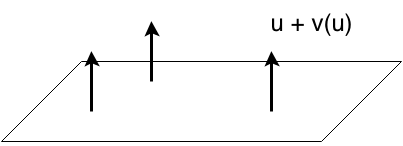
\includegraphics[scale=0.5]{pictures/003-02.png}
\end{center}
\end{definition}

\begin{lemma}
Ist $M\subset\mathbb{R}^n$ eine zusammenhängende Hyperflääche, so existiert entweder \emph{kein} oder \emph{genau zwei} Einheitsnormalenfelder. 
\end{lemma}

\begin{proof}
Als Vorbetrachtung lässt sich sagen, dass wenn $\nu$ ein Einheitsnormalenfeld ist, auch $-\nu$ eins sein muss.\\
Nehmen wir nun an, es gäbe zwei verschiedene Einheitsnormalenfelder $\nu$ und $\tilde{\nu}$. 
Wir können ausnutzen, dass die beiden Felder normiert sind und stellen sofort fest, da $\dim N_uM=1$ ist, dass das Skalarprodukt der beiden nur
\begin{equation*}
s(u)\coloneqq\scap{\nu(u)}{\tilde{\nu}(u)}=\pm 1
\end{equation*}
sein kann. Wir können nun eine weitere wichtige Eigenschaft von $s$ und $M$ ausnutzen.
Da $M$ zusammenhängend und $s$ stetig auf $M$ ist, lässt sich der Zwischenwertsatz zu Hilfe nehmen, 
der uns liefert, dass $s$ für alle $u$ konstant sein \emph{muss}, nämlich entweder $s(u)=1$ oder $s(u)=-1$.
Damit kann $\tilde{\nu}$ nur entweder gleich $\nu$ oder gleich $-\nu$ sein.
\end{proof}

\begin{beispiel}[Möbiusband]
Das wohlbekannte Möbiusband besitzt \emph{kein} Einheitsnormalenfeld.\\
\textbf{grafk fehlt.} 
\end{beispiel}

\begin{beispiel}
Wir betrachten die Konstruktion von Einheitsnormalenfeldern für Hyperflächen $M\coloneqq \{f=0\}$.
Sei $f\in C^1\left(V,\mathbb{R}\right)$ mit $V$ offen und $0$ ein regulärer Wert von $f$. 
Wir können leicht ein Einheitsnormalenfeld definieren und wählen
\begin{equation*}
\nu(u)\coloneqq\frac{f'(u)}{||f'(u)||}
\end{equation*}
\end{beispiel}

Wir wollen nun im folgenden weitere Operationen auf Mannigfaltigkeiten untersuchen.
Im $\mathbb{R}^n$ ist uns das Kreuzprodukt $...\times...$ wohlbekannt.
Es ist zweckmäßig diesen Begriff auf beliege Dimensionen zu verallgemeinern.
\begin{definition}[Äußeres Produkt]
Nehmen wir uns die Vektoren $a_1,a_2,...,a_{n-1}\in\mathbb{R}^n$ und schreiben sie einfach als Spaltenvektoren hintereinander in eine Matrix:
\begin{equation*}
A\coloneqq(a_1|a_2|...|a_{n-1})\in\mathbb{R}^{n\times(n-1)}
\end{equation*}
Wir entfernen nun aus dieser die $k$-te Zeile und nennen sie dann $A_k\in\mathbb{R}^{(n-1)\times(n-1)}$. 
Den Ausdruck
\begin{equation*}
a_1\wedge a_2\wedge...\wedge a_{n-1}\coloneqq\alpha=\begin{pmatrix}
\alpha_1 \\ \alpha_2 \\ \vdots \\ \alpha_k
\end{pmatrix}
\end{equation*}
nennen wir \textbf{äußeres Produkt} von $a_1,a_2,...,a_{n-1}$, wobei
\begin{equation*}
\alpha_k=(-1)^{k-1}\cdot\det A_k
\end{equation*}
\end{definition}
Wir können sofort einige interessante Eigenschaften ablesen, die uns an das bekannte Kreuzprodukt erinnern:
\begin{enumerate}
\item $\alpha$ steht senkrecht auf allen $a_1,a_2,...,a_{n-1}$.
\item Das \emph{Volumen} des von $a_1,a_2,...,a_{n-1}$ aufgespannten Parallelotops  entspricht gerade der Norm $||\alpha||$ des äußeres Produkts.
\end{enumerate}

\begin{beispiel}
Die eben untersuchten Eigenschaften bringen uns dazu, im $\mathbb{R}^3$ das äußerde Produkt mit dem Kreuzprodukt zu identifizieren.
\begin{equation*}
\alpha_1\wedge\alpha_2\equiv\alpha_1\times\alpha_2 \ \ \ \ \ \text{für\ } n=3
\end{equation*}
\end{beispiel}

\begin{lemma}
Sind $b, a_1,a_2,...,a_{n-1}\in\mathbb{R}^n$, so ist
\begin{equation}
\scap{b}{a_1\wedge a_2\wedge...\wedge a_{n-1}}=\det (b | a_1|a_2|...|a_{n-1})
\end{equation}
wobei
\begin{equation*}
a_1\wedge a_2\wedge...\wedge a_{n-1} \ \bot a_i
\end{equation*}
und
\begin{equation*}
a_1\wedge a_2\wedge...\wedge a_{n-1} \ \ \ \ \ \left\{\begin{matrix}
=0 \ \ \text{falls\ }a_i\ \text{linear abhängig} \\
\ \ \ \ \ \neq 0 \ \ \text{falls\ }a_i\ \text{linear unabhängig}
\end{matrix}\right.
\end{equation*}
\end{lemma}

\begin{proof}
Wir können die Determinante in (29.4) nach der 1. Spalte $b$ entwickeln. Aus $b=a_i$ folgen die Bedingungen.
\end{proof}

\begin{beispiel}
Konstruieren wir ein Einheitsnormalenfeld mittels der Parametrisierung $\varphi:V\subset\mathbb{R}^{n-1}\rightarrow\mathbb{R}^n$ mit $V$ offen. 
$M=\{\varphi(v)\}$ sei die entsprechende Hyperfläche. Nach Satz 6 wissen wir, dass $\pdiff{}{x_j}\varphi(x)$ für alle $x$ und für alle $j=1,2,...,n-1$ im Tangentialraum $T_{\varphi(x)}M$ liegt. Wir erkennen außerdem, dass 
\begin{equation*}
N(x)\coloneqq\varphi_{x_1}(x)\wedge\varphi_{x_2}(x)\wedge ... \wedge\varphi_{x_{n-1}}
\end{equation*}
in $N_{\varphi(x)}M$ liegt und können damit
\begin{equation*}
\nu(x)\coloneqq\frac{N(x)}{||N(x)||}
\end{equation*}
als Einheitsnormalenfeld von $M$ wählen. Man beachte, dass $\varphi'(x)$ für alle $x$ regulär ist!
\end{beispiel}
Wir kommen zum Abschluss dieses Kapitels. Wir haben uns mit Mannigfaltigkeiten und ihren Eigenschaften beschäftigt. Als nächstes möchten wir die Integration auf ihnen untersuchen, beschränken uns dabei jedoch noch auf Kartengebiete.

\section{Integration auf Kartengebieten}
Wir stellen uns zunächst die interessante Frage, wie man den Oberflächeninhalt beziehungsweise das d-dimensionale Äquivalent dazu von einer Mannigfaltigkeit bestimmen kann. 
Die Idee wäre natürlich, wie etwa bei der Integration über $\mathbb{R}$, sie durch \emph{ebene} Mannigfaltigkeiten (etwa mit Dreiecken) stückweise zu approximieren.\\
\begin{center}
	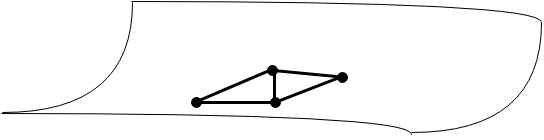
\includegraphics[scale=0.5]{pictures/003-03.png}
\end{center}
\begin{equation*}
\textbf{Fläche}(M)=\sup \sum\limits_\Delta \textbf{Dreiecksflächen}
\end{equation*}
Wir stellen jedoch mit großem Entsetzen schnell fest, dass diese Methode nur für Kurven ($d=1$) funktioniert.\\
\begin{center}
	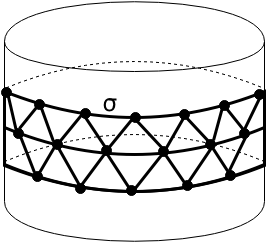
\includegraphics[scale=0.5]{pictures/003-04.png}
\end{center}
Schauen wir uns zum Beispiel eine Zylinderfläche $M\subset\mathbb{R}^3$ an. 
Lassen wir die Feinheit $\sigma$ beliebig klein werden - heute ist ja schließlich alles nano! - so wachsen die Dreiecksflächen immer weiter, 
bis die Fläche von $M$ über alle Grenzen hinaus wächst. Wir müssen uns also wohl sofort wieder von dieser Methode verabschieden.\\
\begin{center}
	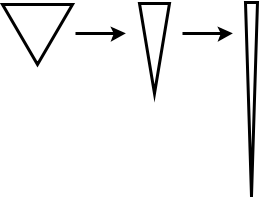
\includegraphics[scale=0.5]{pictures/003-05.png}
\end{center}
\emph{Über dieses Dilemma nachlesen kann man übrigens in Hildebrand, Analysis 2 unter ''Schwartz'scher Stiefel''.}\\
\linebreak
Versuchen wir also etwas neues (für $d=2$) zu finden. Wir nehmen hierzu tangentionale Parallelogramme (äußere Approximation).
$\varphi'(x):\mathbb{R}^d\rightarrow\mathbb{R}^n$ ist linear. Die Methode gestaltet sich also zu
\begin{equation*}
\textbf{Fläche}(M)=\lim\limits_{\sigma\rightarrow 0}\left(\sum\textbf{Fläche\ }\varphi'(x_j)(Q)\right)
\end{equation*}
\begin{center}
	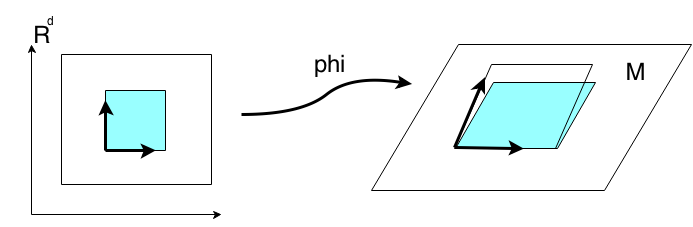
\includegraphics[scale=0.5]{pictures/003-06.png}
\end{center}
\begin{definition}[Parallelotop]
    Seien $a_1, \ldots, a_d \in \mathbb{R}^n (d \leq n)$ \\
    Dann heißt die Menge
    $P \left( a_1, \ldots, a_d \right) \coloneqq 
    \left\lbrace 
    \sum\limits_{j=1}^n t_j a_j | t_j \in [0,1], j = 1, \ldots, d    
    \right\rbrace$ \\
    das von $a_1, \ldots, a_d $ aufgespannte \textbf{Parallelotop} (auch d-Spat genannt).
\end{definition}

\textbf{Einschub:} Eine allgemeine Theorie für d-dimensionale Inhalte liefert das
Hausdorff-Maß $\mathcal{H}^d$, dieses ist jedoch sehr viel abstrakter und schwierig 
'auszurechnen'. Mithilfe von Mannigfaltgkeiten kommt man schneller zu Ergebnissen. \\
Weiterhin ist uns bereits das Maß über die delta-Funktion/Distribution bekannt, welches
zur Beschreibung von Punktmassen und -ladungen wichtig ist.

\begin{satz}
    \mbox{}
    Seien $a_1, \ldots, a_n \in \mathbb{R}^n$, \\
    das aufgespannte Volumen 
    $v(a_1, \ldots , a_n) \coloneqq \mathcal{L}^n (P (a_1, \ldots, a_n))$ \\
    so gilt:
    \begin{enumerate}
        \item[i)]
            $v(a_1, \ldots, \lambda a_k, \ldots, a_n) = 
            |\lambda| v(a_1, \ldots, a_n) \forall \lambda \in \mathbb{R}^n $
        \item[ii)]
            $v(a_1, \ldots, a_k + a_j, \ldots, a_n) = v(a_1, \ldots, a_n) $
            falls $k \neq j $ \\
            Dies ist bekannt als \textit{Prinzip des Cavaleri}, als Veranschaulichung kann
            ein Stapel Spielkarten dienen: Egal wie man eine Seitenfläche von einem Rechteck
            in ein Parallelogramm (oder umgekehrt) verschiebt, 
            das Volumen des Stapels bleibt gleich. \\
            \textbf{Skizze fehlt}
        \item[iii)]
            $v(a_1, \ldots, a_n) = 1 $ falls $a_1, \ldots, a_n $ ein Orthonormalsystem
            in $\mathbb{R}^n $ bilden. \\
            (Der Parallelotop ist dann der Einheitswürfel.)
        \item[iv)]
            $v(a_1, \ldots, a_n) = |\det A|$ für $A \coloneqq (a_1 | \ldots | a_n) $ \\
            Das heißt die Determinante der Matrix mit den Spaltenvektoren $a_1, \ldots, a_n$
            liefert das Volumen des aufgespannten Parallelotops. (Vgl. lin. Algbebra)
    \end{enumerate}
\end{satz}

    \textbf{Beachte:} Die Eigenschaften i) - iii) implizieren bereits iv), die Argumentation
    dazu verläuft wie zu den aus LAG bekannten Eigenschaften der Determinante, vgl.
    auch die axiomatische Definition der Determinante.

\begin{proof}
    \mbox{}
    \begin{enumerate}
        \item[a)] 
            Angenommen, $a_1, \ldots, a_n$ sind linear abhängig. \\
            Dann ist das aufgespannte Parallelotop 'flach', da es in mindestens 
            einer Dimension an Ausdehnung fehlt.
            $\Rightarrow v(a_1, \ldots, a_n) = 0 $ \\
            $\Rightarrow $ iv) ist korrekt 
            (da die Determinante einer singulären Matrix Null ist) \\
            $\Rightarrow $ i) und ii) sind korrekt
        \item[b)]
            Angenommen, $a_1, \ldots, a_n$ sind linear unabhängig. \\
            Sei $\lbrace e_1, \ldots, e_n \rbrace$ die Standard-Orthonormalbasis in
            $\mathbb{R}^n $, dafür gilt iii) nach der Definition des Lebesgue-Maß
            (Es ist ein Quader mit allen Seitenlängen gleich Eins). \\
            Weiter seien nun $U \coloneqq P(e_1, \ldots, e_n),
            V \coloneqq P(a_1, \ldots, a_n) $ \\
            $\Rightarrow A: \mathrm{int}\ U \rightarrow \mathrm{int}\ V $
            ist ein Diffeomorphismus (A ist regulär, ist damit differenzierbar und
            besitzt ein differenzierbares Inverses). \\
            Offenbar ist $A'(y) = A \forall y $ \\
            $\xRightarrow{\text{Trafosatz, Kap. 24}}
            \mathcal{L}^n (V) = \int\limits_V \mathrm{d}x \stackrel{y = Ax}{=}
            \int\limits_U |\det A| \mathrm{d}y = |\det A| \underbrace{\mathcal{L}^n (U)}_1
            = |\det A|
            \Rightarrow $ iv) $\Rightarrow $ i), ii), iii) folgen als Eigenschaften
            der Determinanten
    \end{enumerate}
\end{proof}

\textbf{Ziel:} Bestimmung des d-dimensionalen Inhalts 
$v_d (P(a_1, \ldots, a_d))$ in $\mathbb{R}^n $
\textbf{Idee:} Betrachte $P(a_1, \ldots, a_n)$ als Teilmenge eines d-dimensionalen
Vektorraums $X$ und nimm das d-dimensional Lebesgue-Maß in $X$.\\
Somit sollte $v_d: 
\underbrace{\mathbb{R}^n \times \ldots \times \mathbb{R}^n }_{\text{d-mal}}
\rightarrow \mathbb{R}_{\geq 0} $
folgende Eigenschaften haben:
\begin{enumerate}
    \item[(v1)]
        $v_d (a_1, \ldots, \lambda a_k, \ldots, a_d) = |\lambda| v_d(a_1, \ldots, a_d)
        \forall \lambda \in \mathbb{R} $
    \item[(v2)]
        $v_d (a_1, \ldots, a_k + a_j, \ldots, a_d) = v_d(a_1, \ldots, a_d) $
        falls $k \neq j$ (Prinzip des Cavaleri)
    \item[(v3)]
        $v_d(a_1, \ldots, a_d) = 1 $ falls $\lbrace a_1, \ldots, a_d \rbrace $
        orthonormal zueinander sind.
\end{enumerate}

\begin{satz}
    $v_d$ ist durch (v1), (v2), (v3) eindeutig bestimmt, und es gilt:
    \begin{equation}
        v_d(a_1, \ldots, a_d) = 
        \sqrt[]{\det \underbrace{A^T A}_{\in \mathbb{R}^{d \times d}}}
        \text{ mit } 
        A \coloneqq\underbrace{(a_1 | \ldots | a_d)}_{\in \mathbb{R}^{n \times d}}
    \end{equation}
\end{satz}

\textbf{Bemerkung:}
\mbox{}
\begin{enumerate}
    \item
        für $d=n $ liefert (30.1) Gleichung iv) in Satz 1
    \item
        $A^T A $ ist stets symmetrisch und positiv definit
        $\left( \left\langle x, A^T Ax \right\rangle =
        \langle Ax, Ax \rangle = \|Ax\|^2 \geq 0 \right)$
        und somit ist auch stets $\det A^T A \geq 0 $
    \item
        $v_d (a_1, \ldots, a_d) = 0 \Leftrightarrow a_1, \ldots, a_d$ linear abhängig
\end{enumerate}

\begin{proof}
    Selbststudium, verwende:\\
    $A^T A = 
    \begin{pmatrix}
        \alpha_{11} & \ldots & \alpha_{1n} \\
        \vdots      & \ddots & \vdots \\
        \alpha_{n1} & \ldots & \alpha_{nn}
    \end{pmatrix}
    $mit $\langle a_i, a_j \rangle $ \\
    und argumentiere wie bei den Eigenschaften der Determinante.
\end{proof}

\begin{beispiel}
    $d = n-1 $: Sei $a_1, \ldots, a_{n-a} \in \mathbb{R}^n, 
    a \coloneqq a_1 \wedge \ldots \wedge a_{n-1} $
    \begin{equation}
        \Rightarrow v_{n-1} (a_1, \ldots, a_{n-1}) = |a|_2
    \end{equation}
    Das heißt die euklidische Länge des äußeren Produkts liefert das Volumen.\\
    Denn: $
    \begin{pmatrix}
        a^T \\
        \rule[.5ex]{1em}{1pt}\\
        A^T
    \end{pmatrix}
    \bullet
    \begin{pmatrix}
        a & | & A 
    \end{pmatrix}
    =
    \begin{pmatrix}
        \langle a,a \rangle & 0 \\
        0 & A^T A
    \end{pmatrix}
    $ wegen $\langle a_i, a_j \rangle = 0 \forall j $; $A$ wie in (1)\\
    $\Rightarrow |a|_2^2 \det A^T A = (\det (a|A))^2 \stackrel{(29.4)}{=}
    |a|_2^4 \xRightarrow{\text{(1)}} $ (2)
\end{beispiel}

\textbf{Frage:} Existiert für eine Mannigfaltigkeit $M$ eine Transforamtion, so dass das
Volumen eines Quaders $Q \in \mathbb{R}^d $ auf das eines Parallelotops 
$P \subset T_uM \in \mathbb{R}^n $ abgebildet wird: \\
$v_d(\text{Quader }Q) \xrightarrow{\varphi'(x)} v_d(\text{Parallelotop } P) $ ?\\
\textbf{Skizzen fehlen}\\
Für einen Quader $Q = P(b_1, \ldots, b_d) \subset \mathbb{R}^d $ ist 
$P(a_1, \ldots, a_d) \subset T_uM \in \mathbb{R}^n $ das zugehörige Parallelotop, falls
$a_j = \varphi'(x) b_j $,für $ j=1, \ldots, d $

\begin{satz}
    Sei $M$ eine d-dimensionale Mannigfaltigkeit,\\
    $\varphi$ eine Parametrisierung um $\varphi(x) = u \in M $
    und sei \\
    $Q \coloneqq P(b_1, \ldots, b_d) \subset \mathbb{R}^d $ ein Quader 
    $(b_j \in \mathbb{R}^d),
    a_j \coloneqq \varphi'(x) b_j,\ j= 1, \ldots, d $
    \begin{equation}
        \Longrightarrow 
        v_d(a_1, \ldots, a_d) = 
        \sqrt{\det \varphi'(x)^T \varphi'(x)}\ v_d(b_1, \ldots, b_d)
    \end{equation}
\end{satz}

\begin{definition}[Maßtensor und Gramsche Determinante]
    \mbox{} \\
    $\varphi'(x)^T \varphi'(x) \in \mathbb{R}^{d \times d} $
    heißt \textbf{Maßtensor} von $\varphi$ in $x$ und\\
    $g^\varphi (x) \coloneqq \det \varphi'(x)^T \varphi'(x) $
    heißt \textbf{Gramsche Determinante} von $\varphi$ in $x$.
\end{definition}

\begin{proof}
    Sei $B = (b_1, \ldots, b_d) \in \mathbb{R}^{d \times d},\ 
    A = (a_1, \ldots, a_d) \in \mathbb{R}^{n \times d} \\
    \xRightarrow{\text{(1)}} v_d(a_1, \ldots, a_d) 
    = \sqrt{\det A^T A} = \sqrt{\det ((\varphi'(x) B)^T \varphi'(x) B)}
    = \sqrt{\det \varphi'(x)^T \varphi'(x)} 
    \underbrace{\sqrt{\det B^T B}}_{= v_d(b_1, \ldots, b_d)}
    $
\end{proof}

Sei $M \subset \mathbb{R}^n $ eine d-dimensionale Mannigfaltigkeit,
$\varphi: V \rightarrow U $ eine lokale Parametriesierung,
$f: \rightarrow \mathbb{R} $ eine Funktion auf dem Kartengebiet $U$.\\
Motiviert durch die Riemann-Summen (Kap. 22)\\
$\sum f(u_i) v_d(P_i) = \sum f(\varphi(x_i)) \sqrt{g^\varphi (x_i)} v_d(Q_i) $
mit $P_i = \varphi'(x_i) Q_i $
definieren wir:

\begin{definition}[Integral über über Kartengebiet]
    \begin{equation}
        \int\limits_U f \mathrm{d}a 
        \coloneqq \int\limits_V f(\varphi(x)) \sqrt{g^\varphi (x)} \mathrm{d}x
    \end{equation}
    als \textbf{Integral von $f$} über das Kartengebiet $U$ falls die rechte
    Seite existiert.\\
    $f$ heißt dann \textbf{integrierbar} auf $U$.
\end{definition}

\textbf{Bemerkung:}
\begin{enumerate}
    \item[-]
        die rechte Seite in (30.4) ist ein Lebesgue-Integral in $\mathbb{R}$
    \item[-]
        damit die Definition von (30.4) sinnvoll ist, sollte die rechte Seite
        unabhängig von $\varphi$ sein
    \item[-]
        mittels des Hausdorff-Maß $\mathcal{H}^d $ kann
        $\int\limits_U f \mathrm{d}a $
        völlig analog zum Lebesgue-Maß definiert werden
        $\left(\int\limits_U f(u) \mathrm{d} \mathcal{H} (u) \right) $
    \item[-]
        für n-dimensionale Mannigfaltigkeiten $M \subset \mathbb{R}^n: \\
        \int\limits_U f \mathrm{d}a = $ Lebesgue-Integral 
        $\int\limits_U f \mathrm{d}x $ falls dieses existiert
\end{enumerate}

\begin{satz}
    Sei $M \subset \mathbb{R}^n $ eine d-dimensionale Mannigfaltigkeit,\\
    $U \subset M $ ein Kartengebiet, $f:U \rightarrow \mathbb{R} $ und
    $\varphi_i: V_i \rightarrow U,\ i=1,2 $ seien zugehörige Parametrisierungen. \\
    $\Longrightarrow \int\limits_{V_1} f(\varphi_1(x)) \sqrt{g^{\varphi_1} (x)} \mathrm{d}x
    = \int\limits_{V_2} f(\varphi_2(x)) \sqrt{g^{\varphi_2} (x)} \mathrm{d}x
    $ falls ein Integral exisitiert.
\end{satz}

\textbf{Somit:} (4) ist unabhängig von der Parametrisierung
\begin{equation}
    f(.) \text{ int'bar auf } U
    \Longleftrightarrow f(\varphi(.)) \sqrt{g^\varphi (x)} 
    \text{ int'bar auf } V
    \text{ für eine Param. }
    \varphi: V \rightarrow U
\end{equation}

\begin{proof}
    $\psi \coloneqq \varphi_1^{-1} \bullet \varphi_2: V_2 \rightarrow V_1 $
    ist ein Diffeomorphismus nach Lemma 5 \\
    $\xRightarrow{\text{Trafosatz}} 
    \int\limits_{V_1} f(\varphi_1(x)) \sqrt{g^{\varphi_1} (x)} \mathrm{d}x
    \stackrel{x=\psi(y)}{=}
    \int\limits_{V_2} f(\varphi_1(\psi(y)))
    \underbrace{
        \sqrt{\det \varphi_1'(\psi(y))^T \varphi_1'(\psi(y))}
        \underbrace{
            |\det \psi'(y)|
            }_{
            = \sqrt{\det \psi'(y)^T \psi'(y)}}
        }_{
        = \sqrt{\det \psi'^T \varphi_1'^T \psi' \varphi_1'}
        = \sqrt{\det (\psi' \varphi_1')^T \psi' \varphi_1'}
        }
    \mathrm{d}y
    $ wegen $
    \varphi_2 (y) = \varphi_1 (\psi(y))
    \xRightarrow{\text{Kettenregel}}
    \varphi_2' (y) = \varphi_1' (\psi(y)) \psi'(y)
    \Rightarrow $ Behauptung.
\end{proof}
Nehmen wir uns die Funktion $f\equiv 1$ her, 
die offensichtlich integrierbar auf jedem Kartengebiet $U\subset M$ ist, 
dann ist
\begin{equation}
	v_d(U)\coloneqq \int_U 1 \mathrm{d}a 
	\ \ \left( =\int_V 1 \sqrt{g^\varphi(x)}\mathrm{d}x\right)
\end{equation}
der d-dimensionale Inhalt (Maß, Länge, Fläche, Volumen,...) von $U$ 
wobei $\sqrt{g^\varphi(x)}$ das Flächenelement von $U$ bezüglich $\varphi$ ist.\\
Mit dieser Definition entspricht $v_d(U)\equiv\mathcal{H}^d(U)$ direkt 
mit dem d-dimensionalen Hausdorffmaß überein (siehe Literatur).\\
Wir stellen außerdem nach (30.4) fest, dass $v_d(U)$ genau dann verschwindet, 
wenn $U$ ein Nullmenge ist:
\begin{equation*}
	v_d(U)=0 \ \Leftrightarrow \ \mathcal{L}^d(\varphi^{-1}(U))=0
\end{equation*}

\begin{beispiel}
Wir wollen $\int_Mf\mathrm{d}a$ auf einer Halbsphäre mit Radius $r$, 
gegeben durch
\begin{equation*}
	M\coloneqq\left\{u=(u_1,u_2,u_3)\in\mathbb{R}^3\middle| ||u||=r, u_1>0\right\}
\end{equation*}
berechnen und parametrisieren $M$ dafür in Kugelkoordinaten durch
\begin{equation*}
	\varphi(x_1,x_2)=r\begin{pmatrix}
	\cos x_1 \cos x_2 \\ \cos x_2 \sin x_1 \\ \sin x_2
	\end{pmatrix}
	\ \ \text{für\ } (x_1,x_2)\in V\coloneqq \left(-\frac{\pi}{2},\frac{\pi}{2}\right)^2
\end{equation*}
Offenbar ist $\varphi:V\rightarrow M$ stetig differenzierbar, regulär und homöomorph. 
Es handelt sich also tatsächlich um eine echte Parametrisierung von $M$. 
Das macht natürlich $M$ zu einer Mannigfaltigkeit und sogar zu einem Kartengebiet.
Um das Volumen zu berechnen benötigen wir zunächst
\begin{equation*}
	\varphi'(x)=r\begin{pmatrix}
	-\cos x_2 \sin x_1 & -\sin x_2 \cos x_1 \\
	 \cos x_2 \cos x_1 & -\sin x_2 \sin x_1 \\
	 0 & \cos x_2
	\end{pmatrix}
\end{equation*}
um über 
\begin{equation*}
	\varphi'(x)^T\varphi'(x)=r^2\begin{pmatrix}
	\cos^2 x_2 & 0 \\ 0 & 1 
	\end{pmatrix}
\end{equation*}
das Flächenelement
\begin{equation*}
	\sqrt{g^\varphi(x)}=r^2\cos x_2
\end{equation*}
zu berechnen.\\
Damit können wir das zu berechnende Integral folgendermaßen ausdrücken:
\begin{equation*}
	\int_Mf\mathrm{d}a = r^2\int_Vf(\varphi(x))\cos x_2\mathrm{d}x = 
	r^2\int\limits_{-\frac{\pi}{2}}^{\frac{\pi}{2}}\cos x_2\int\limits_{-\frac{\pi}{2}}^{\frac{\pi}{2}}f(\varphi(x)\mathrm{d}x_1\mathrm{d}x_2 
\end{equation*}
Wählen wir nun zum Beispiel $f(u)=u_1^2+u_2^2$, dann ist $f(\varphi(x)=r^2\cos^2 x_2$ und das Integral wird zu
\begin{equation*}
	\int_M(u_1^2+u_2^2)\mathrm{d}a=r^4\int\limits_{-\frac{\pi}{2}}^{\frac{\pi}{2}}\cos x_2 \int\limits_{-\frac{\pi}{2}}^{\frac{\pi}{2}}\mathrm{d}x_1\mathrm{d}x_2 =
\end{equation*}
\begin{equation*}
	= \pi r^4 \int\limits_{-\frac{\pi}{2}}^{\frac{\pi}{2}} \cos^3 x_2\mathrm{d}x_2 = \pi r^4 \left[\sin x_2-\frac{1}{3}\sin^3 x_2\right]_{-\frac{\pi}{2}}^{\frac{\pi}{2}} = 
	2\pi r^4\left(1-\frac{1}{3}\right)=\frac{4}{3}\pi r^4
\end{equation*}
Ist nun $f(u)=1$, dann ist
\begin{equation*}
	v_d(M)=\pi r^2 \int_M\mathrm{d}a=\pi r^2 \int\limits_{-\frac{\pi}{2}}^{\frac{\pi}{2}} \cos x_2 \mathrm{d}x_2 = 
	\pi r^2 \left[\sin x_2\right]_{-\frac{\pi}{2}}^{\frac{\pi}{2}} = 2 \pi r^2
\end{equation*}
was genau genau der halben Sphärenfläche entspricht. 
Es ist zu bemerken, dass wir in unserer Rechnung den Rand von $M$ komplett vernachlässigt haben. 
Wir werden jedoch später zeigen, dass derartige Nullmengen keinen Beitrag leisten. 
\end{beispiel}

\begin{satz}[Integral über $(n-1)$-dimensionale Graphen]
\ \\ Sei $g:V\subset\mathbb{R}^{n-1}\rightarrow\mathbb{R}$ mit $V$ offen eine stetig differenzierbare Funktion und 
\begin{equation*}
	\Gamma\coloneqq\left\{\left(x,g(x)\right)\in\mathbb{R}^n \middle| x\in V \right\}
\end{equation*}
der Graph von $g$. Dann gilt für $f:\Gamma\rightarrow\mathrm{R}$
\begin{equation}
\int_\Gamma f\mathrm{d}a=\int_Vf\left(x,g(x)\right)\sqrt{1+|g(x)|^2}\mathrm{d}x
\end{equation}
falls die rechte Seite existiert.
\end{satz}

\begin{proof}
$\Gamma$ ist eine $(n-1)$-Mannigfaltigkeit (vgl. Bsp. 29.2) 
und auch Kartengebiet bezüglich der Parametrisierung $\varphi:V\rightarrow\Gamma$ 
mit $\varphi(x)=\left(x,g(x)\right)$. Wir setzen 
\begin{equation*}
	\gamma\coloneqq\sqrt{\det \varphi'(x)^T\varphi'(x)}
\end{equation*}
und sehen mit (30.1), dass
\begin{equation*}
	\gamma=v_{n-1}\left(\varphi_{x_1}(x)\middle|...\middle|\varphi_{x_{n-1}}(x)\right)
\end{equation*}
und dann wiederum mit (30.2)
\begin{equation*}
	\gamma=||\varphi_{x_1}(x)\wedge ... \wedge \varphi_{x_{n-1}}(x)||
\end{equation*}
Da aber auch
\begin{equation*}
	\varphi_{x_1}(x)\wedge ... \wedge \varphi_{x_{n-1}}(x)=(-1)^n\begin{pmatrix}
	g'(x) \\ -1
	\end{pmatrix}\in\mathbb{R}^n
\end{equation*}
gilt, können wir $\gamma$ auch als
\begin{equation*}
	\gamma=\sqrt{1+||g'(x)||^2}
\end{equation*}
schreiben. Damit erhalten wir
\begin{equation*}
	\int_\Gamma f\mathrm{d}a=\int f(\varphi(x))\sqrt{1+||g'(x)||^2}\mathrm{d}x
\end{equation*}
falls die rechte Seite existiert. Damit gilt für den Inhalt von $\Gamma$ (falls er existiert):
\begin{equation}
	v_{n-1}(\Gamma)=\int_V\sqrt{1+||g'(x)||^2}\mathrm{d}x
\end{equation}
\end{proof}

\begin{beispiel}
Betrachten wir die Halbsphäre
\begin{equation*}
	S_+^{n-1}\coloneqq\left\{ x\in\mathbb{R}^n \middle| |x|=1,\ x_n>0 \right\}
\end{equation*}
die offenbar für alle $x\in B_1(x)\subset\mathbb{R}^{n-1}$ der Graph von $g(x)=\sqrt{1-|x|^2}$ ist. 
Mit (30.8) sehen wir sofort
\begin{equation*}
	v_{n-1}\left(S_+^{n-1}\right)=\int\limits_{B_1(0)\subset\mathbb{R}^{n-1}}\sqrt{1+\frac{|x|^2}{1-|x|^2}}\mathrm{d}x = \int\limits_{B_1(0)}\frac{1}{\sqrt{1+|x|^2}}\mathrm{d}x
\end{equation*}
Wir können an dieser Stelle ohne Beweis annehmen, dass $f$ rotationssymetrisch auf $B_1(0)\subset\mathbb{R}^{n-1}$ ist (d.h. $f(x)=f(|x|)\ $). Dann verwenden wir (aus Königsberger Analysis 2, Kap 8.2)
\begin{equation}
	\int\limits_{B_r(0)}f(x)\mathrm{d}x = 
	n\kappa_n \int\limits_0^r\tilde{f}(\rho)\rho^{n-1}\mathrm{d}\rho
	\ \ \ \ \ \text{für\ }B_r(0)\subset\mathbb{R}^n \ 	\text{und\ } \kappa_n\coloneqq\mathcal{L}^n \left(B_r(0)\right)
\end{equation}
und münzen dies auf $(n-1)$ um:
\begin{equation*}
	v_{n-1}\left(S_+^{n-1}\right) =
	(n-1)\kappa_{n-1}\int\limits_0^1\frac{r^{n-2}}{\sqrt{1-r^2}}\mathrm{d}r = 
	(n-1)\kappa_{n-1}\int\limits_0^1 r^n\frac{1}{r^2\sqrt{1-r^2}}\mathrm{d}r = 
\end{equation*}	
Dies integrieren wir partiell und erhalten
\begin{equation*}
	= n(n-1)\kappa_{n-1}\int\limits_0^1 r^{n-1}\frac{\sqrt{1-r^2}}{r}\mathrm{d}r=n\int\limits_{B_1(0)}\sqrt{1-|x|^2}\mathrm{d}r=\frac{n}{2}\kappa_n
\end{equation*}	
Was haben wir damit herausbekommen? Wir setzen
\begin{equation*}
	\omega\coloneqq\left(S^{n-1}\right)=2v_{n-1}\left(S_+^{n-1}\right)
\end{equation*}
als die Oberfläche der Sphäre $S^{n-1}\subset\mathbb{R}^n$ und sehen, dass für alle $n\in\mathbb{N}_{\geq 2}$
\begin{equation}
	\omega_n=n\kappa_n
\end{equation}
Das ist ein erstaunliches Resultat, welches wir uns an zwei Beispielen verdeutlichen wollen.\\
\begin{center}
$\begin{matrix}
n=2: & \ \ \ \ \ \  & v_{n-1} & = & 2\pi & = & 2\cdot v_n & = & 2 \cdot \pi \\
n=3: & \ \ \ \ \ \  & v_{n-1} & = & 4\pi & = & 3\cdot v_n & = & 3 \cdot \frac{4}{3}\pi
\end{matrix}$
\end{center}
Wir können dieses Resultat sogar auf beliebige Kugeln skalieren:
\begin{equation*}
	v_n\left(B_r(0)\right)=\mathcal{L}^n\left(B_r(0)\right)=r^n\kappa_n
\end{equation*}
Mithilfe des Transformationssatzes können wir das ganze sogar noch umschreiben 
und erhalten ein Beziehung die sich später in der Differentialgleichungstheorie 
als maßgeblich herausstellen wird:
\begin{equation*}
	v_{n-1}\left(\partial B_r(0)\right)=r^{n-1}\omega_n=r^{n-1}n\kappa_n
\end{equation*}
\end{beispiel}

\begin{beispiel}[Kurvenintegral]
Wir betrachten die Kurve $\varphi:I\subset\mathbb{R}\rightarrow\mathbb{R}^n$, 
wobei $I$ ein offenes Intervall ist, so dass
\begin{equation*}
	C\coloneqq\varphi(I)
\end{equation*}
eine 1-dimensionale Mannigfaltigkeit ist. Wir erinnern uns, dass $\varphi$ 
genau dann regulär ist, wenn $\varphi'(t)\neq 0$ ist. Offenbar ist 
\begin{equation*}
	\det \varphi'(t)^T\varphi'(t)=|\varphi'(t)|^2
\end{equation*}
und so können wir, falls es existiert, für ein $f:C\rightarrow\mathbb{R}$ 
mit $I=(a,b)$ formulieren
\begin{equation}
 \int_Cf\mathrm{d}a=\int\limits_a^bf(\varphi(t))|\varphi'(t)|\mathrm{d}t
\end{equation}
Dieses Integral nennen wir das Kurvenintegral von $f$ entlang des Weges $C$. 
Auf diesem Wege können wir natürlich auch den 1-dimensionalen Inhalt, $C$ 
, den wir \textbf{Bogenlänge} nennen, bestimmen, in dem wir einfach $f\equiv 1$ setzen.
\begin{equation}
	v_1(C)=\int\limits_a^b|\varphi'(t)|\mathrm{d}t
\end{equation}
Falls wir nun noch ein $\varphi$ finden, sodass $|\varphi'(t)|=1$ ist, 
dann nennen wir dieses $\varphi$ \textbf{Bogenlängenparametrisierung} 
von $C$, da uns in diesem Fall $t$ direkt die Bogenlänge liefet:
\begin{equation*}
	t_2-t_1=v_1(\varphi(t_2-t_1))
\end{equation*}
Wir können natürlich auch durch einen Kartenwechsel umparametrisieren 
und erhalten so für 
\begin{equation*}
	\sigma(s)=\int\limits_a^s|\varphi'(t)|\mathrm{d}t 
	\tag{$\ast$}
\end{equation*}
immer ein $\psi:(0,v_s(C))\rightarrow\mathbb{R}^n$ finden, 
das mit $\psi(I)=\varphi(\sigma^{-1}(I))$ stets eine Bogenlängenparametrisierung 
ist. Das können wir ganz leicht zeigen:\\
Offenbar ist $\sigma$ stetig differenzierbar und sogar monoton wachsend, 
weil $\varphi'$ regulär ist. Das bedeutet, dass ein $\sigma^{-1}$ 
existiert, das ebenfalls stetig differenzierbar ist. 
So können wir folgern
\begin{equation*}
	|\psi'(\tau)| = 
	\left| \varphi' ( \sigma^{-1} (\tau)\cdot\sigma^{-1'} (\tau)\right|= 
	\left| \varphi' ( \sigma^{-1}\right|\frac{1}{|\sigma'(\sigma^{-1}(\tau))|} 
	\overset{(\ast)} = 1
\end{equation*}
Für jede Kurve existiert also \emph{genau eine} ausgezeichnete Parametrisierung, 
nämlich die Bogenlängenparametrisierung.
\end{beispiel}
Wir wollen uns dem Thema der Kurvenlänge nun auf eine etwas andere Weise annähern.
\begin{definition}[Rektifizierbarkeit]
Für eine beliebige stetige Funktion $\varphi:[a,b]\rightarrow\mathbb{R}^n$ 
heißt die zugehörige Kurve $C=\varphi([a,b])$ \textbf{rektifizierbar}, 
falls 
\begin{equation*}
	l(C)\coloneqq\sup_Z\left\{\sum\limits_{j=1}^k |\varphi(t_j)-\varphi(t_{j-1})| \middle| \{t_0,...,t_k\}\in Z\right\} < \infty
\end{equation*}
wobei $Z$ die Menge alle geordneten Zerlegungen von $C$ ist. 
Man kann $C$ also eine Länge zuordnen.
\end{definition}

\begin{satz}[Rektifizierbare Kurven]
Sei $\varphi:[a,b]\rightarrow\mathbb{R}^n$ eine 
stetig differenzierbare Funktion, dann ist 
\begin{enumerate}
	\item $\varphi$ rektifizierbar und
	\item $C\coloneqq\varphi((a,b))$ eine 1-dimensionale Mannigfaltigkeit 
	mit der zugehörigen Parametrisierung $\varphi$.
\end{enumerate}
Insbesondere gilt dann:
\begin{equation*}
	l(C)=v_1(C)=\mathcal{H}^1(C)
\end{equation*}
\end{satz}

Das ist beruhigend. Wir möchten uns den gesamten Beweis ersparen, dann 
er mit sehr viel Schreibarbeit verbunden ist. Deshalb hier nur eine 
\emph{Beweisskizze}:\\
$\varphi$ ist Lipschitz-stetig auf $[a,b]$, also 
\begin{equation*}
	l(\varphi[a,b])<L[a,b]
\end{equation*}
Damit ist $\varphi$ rektifizierbar und 1. gezeigt. Für 2. zeigen wir, dass
\begin{equation*}
	l(t)\coloneqq l(\varphi[a,t])<L[a,b] 
\end{equation*}
stetig differenzierbar auf $(a,b)$ mit $l'(t)=|\varphi'(t)|$ ist. 
Daraus folgt dann 
\begin{equation*}
	l(b)=\int\limits_a^bl'(t)\mathrm{d}t = 
	\int\limits_a^b|\varphi'(t)|\mathrm{d}t = 
	v_1(C)
\end{equation*}

\begin{beispiel}[Umfang des Einheitskreises]
\begin{equation*}
	\varphi:\left(-\pi,\pi\right)\rightarrow\mathbb{R}^n 
	\ \ \ \ \ \text{mit\ } \varphi(t)=\begin{pmatrix}
	\cos t \\ \sin t
	\end{pmatrix}
\end{equation*}
$C\coloneqq \varphi([-\pi,\pi])$ ist der Einheitskreis ohne den Punkt $(-1,0)^T$. 
Dann ist 
\begin{equation*}
	v_1(C)=\int\limits_{-\pi}^{\pi}|\varphi'(t)|\mathrm{d}t=\int\limits_{-\pi}^{\pi}\left\|\begin{pmatrix}
	-\sin x \\ \cos x
	\end{pmatrix}\right\|\mathrm{d}t = 
	\int\limits_{-\pi}^{\pi}1\mathrm{d}t=2\pi
\end{equation*}
Wichtig hierbei ist, dass $\pi$ die Bogenparametrisierung ist.
\end{beispiel}

\end{document}